\documentclass[12pt,twoside, a4paper, twocolumn]{article}
\usepackage[utf8]{inputenc}
\usepackage[brazil]{babel}
\usepackage[margin = 0.5in]{geometry}
\usepackage{amsmath}
\usepackage{amsthm}
\usepackage{amssymb}
\usepackage{amsthm}
\usepackage{setspace}
\usepackage[americanvoltages,fulldiodes,siunitx]{circuitikz}
\usepackage{lipsum}
\usepackage{pgfplots}
\usepackage{ifthen}
\usepackage{adjustbox}
\usepackage[section]{placeins}
\usepackage{hyperref}
\usepackage{graphicx}
\usepackage{amsmath}
\usepackage{amsthm}
\usepackage{amssymb}
\usepackage{amsthm}
\usepackage{setspace}
\usepackage[americanvoltages,fulldiodes,siunitx]{circuitikz}
\usepackage{lipsum}
\usepackage{pgfplots}
\usepackage{ifthen}
\usepackage{adjustbox}
\usepackage[section]{placeins}
\usepackage{hyperref}
\usepackage{graphicx}
\usepackage{adjustbox}
\pgfplotsset{compat=newest}
\graphicspath{ {./images/} }
%  #1 color - optional #2 x_0 #3 y_0 #4 x_f #5 y_f #6 name - optional  #7 true if adding lines to axis
\newcommand{\drawvector} [9] [color=cyan] {
\draw[line width=1.5pt,#1,-stealth](axis cs: #2, #3)--(axis cs: #4, #5) node[anchor=south west]{$#6$};
\ifthenelse{\equal{#7}{true}}{
\draw[line width=1pt,#1, dashed](axis cs: #4, #5)--(axis cs: #4, 0) node[anchor= north west]{$#8$};
\draw[line width=1pt,#1, dashed](axis cs: #4, #5)--(axis cs: 0, #5) node[anchor=south east]{$#9$};
}
{}
}
\newcommand\deriv[2]{\frac{\mathrm d #1}{\mathrm d #2}}
\title{Terceiro Relatório de Lab de Circuitos II}
\author{Henrique da Silva \\ hpsilva@proton.me}
\date{\today}
\pgfplotsset{width = 10cm, compat = 1.9}
\begin{document}
\maketitle
\pagenumbering{gobble}
\newpage
%pagenumbering{roman}
\tableofcontents
\newpage


\section{Introdução}


\subparagraph*{Neste relatório, vamos discutir filtros passa-baixa, e como utilizar um amp op como buffer de corrente para reduzir o efeito da carga no filtro.}


\subparagraph*{Todos arquivos utilizados para criar este relatório, e o relatorio em si estão em:  \url{https://github.com/Shapis/ufpe_ee/tree/main/5th semester/Circuits II/}}




\section{Análise preliminar}


\paragraph*{Utilizarei o Maxima para fazer a análise teórica do circuito antes de montá-lo fisicamente.}


\paragraph*{Após terminar as análises compararei os resultados obtidos nas análises numéricas e em laboratório para verificar sua coerência.}


\subsection{Os circuitos}


\subsubsection{Circuito 1}
\begin{adjustbox}{scale=0.6}
    \includegraphics{circuito1.png}
\end{adjustbox}


\subsubsection{Circuito 2}
\begin{adjustbox}{scale=0.6}
    \includegraphics{circuito2.png}
\end{adjustbox}




\subsubsection{Circuito 3}
\begin{adjustbox}{scale=0.6}
    \includegraphics{circuito3.png}
\end{adjustbox}


\subparagraph*{}


\subsection{Maxima}


\subsubsection{Análise do circuito 1}


\subparagraph*{Primeiro fiz manualmente a análise de circuito que vamos construir, utilizei um divisor de tensão, passei o circuito para o domínio da frequência e fiz a função transferência.}
\subparagraph*{}


\begin{adjustbox}{scale=0.4}
    \includegraphics{eqs1.png}
\end{adjustbox}




\subparagraph*{Para obter o ganho vi o que acontecia com a função transferência quando a frequência tendia a zero.}
\subparagraph*{}
\begin{adjustbox}{scale=0.4}
    \includegraphics{ganho1.png}
\end{adjustbox}
\subparagraph*{Podemos ver que quando o $s$ tender a $0$, o ganho tenderá a $1$.}


\subparagraph*{Ja da função transferência observamos que a frequência de corte eh $\frac{1}{RC}$}


\subparagraph*{Logo para projetar um filtro que tenha frequência de corte $50Hz$ fazemos:}


\begin{equation*}
    \begin{aligned}
         &  & 2  \pi f = \frac{1}{RC} \\
         &  & f = 2 \frac{1}{RC \pi}
    \end{aligned}
\end{equation*}


\subparagraph*{Resolvendo para $f = 50Hz$ e $C = 100nF$ temos:}
\subparagraph*{}
\begin{adjustbox}{scale=0.4}
    \includegraphics{freqcorte1.png}
\end{adjustbox}


\subparagraph*{O valor da resistência está próximo ao resistor comercial de $33k \varOmega$.}


\subparagraph*{Utilizando o resistor de $33k \varOmega$, obtemos uma nova frequência de corte de $f = 48Hz$.}




\subparagraph*{E por fim, geramos o diagrama de Bode do ganho do circuito}


\begin{figure}[h]
    \centering
    \includegraphics[width=1\columnwidth]{images/bodegain1.png}
    \caption{Magnitude de H(s) do circuito 1.}
\end{figure}




\subsubsection{Análise do circuito 2}






\subparagraph*{Primeiro fiz manualmente a análise nodal do circuito que vamos construir, passei o circuito para o domínio da frequência e fiz a função transferência.}
\subparagraph*{}


\begin{adjustbox}{scale=0.4}
    \includegraphics{eqs2.png}
\end{adjustbox}




\subparagraph*{Para obter o ganho vi o que acontecia com a função transferência quando a frequência tendia a zero.}
\subparagraph*{}
\begin{adjustbox}{scale=0.4}
    \includegraphics{ganho2.png}
\end{adjustbox}
\subparagraph*{Podemos ver que quando o $s$ tender a $0$, o ganho tenderá a $\frac{2}{5}$.}


\subparagraph*{Com o ganho em mãos podemos achar a frequência $w$, fazendo o seguinte:}


\begin{equation*}
    Ganho = \frac{ | H(jw) |}{\sqrt[]{2}} = \frac{2}{5}
\end{equation*}


\begin{adjustbox}{scale=0.4}
    \includegraphics{freqcorte2.png}
\end{adjustbox}


\subparagraph*{Achamos uma nova frequência de corte de $120Hz$, podemos observar que adicionando a carga, a nossa frequência de corte foi alterada.}


\subparagraph*{E por fim, geramos o diagrama de Bode do ganho do circuito}


\begin{figure}[h]
    \centering
    \includegraphics[width=1\columnwidth]{images/bodegain2.png}
    \caption{Magnitude de H(s) do circuito 2.}
\end{figure}


\subsubsection{Análise do circuito 3}


\subparagraph*{Observamos que neste caso, as equações que regem o circuito, são as mesmas do circuito 1. Já que o terra virtual, isola as duas partes do circuito. Insulando a carga de afetar o seu comportamento. Logo, não haverá $R_L$ na sua função transferência.}


\subparagraph*{Fiz manualmente a análise do circuito que vamos construir, utilizei um divisor de tensão, passei o circuito para o domínio da frequência e fiz a função transferência.}
\subparagraph*{}


\begin{adjustbox}{scale=0.4}
    \includegraphics{eqs1.png}
\end{adjustbox}




\subparagraph*{Para obter o ganho vi o que acontecia com a função transferência quando a frequência tendia a zero.}
\subparagraph*{}
\begin{adjustbox}{scale=0.4}
    \includegraphics{ganho1.png}
\end{adjustbox}
\subparagraph*{Podemos ver que quando o $s$ tender a $0$, o ganho tenderá a $1$.}


\subparagraph*{Ja da função transferência observamos que a frequência de corte eh $\frac{1}{RC}$}




\subparagraph*{Observamos que este circuito  tem exatamente a mesma frequência de corte e ganho do circuito 1.}




\subparagraph*{E por fim, geramos o diagrama de Bode do ganho do circuito}


\begin{figure}[h]
    \centering
    \includegraphics[width=1\columnwidth]{images/bodegain1.png}
    \caption{Magnitude de H(s) do circuito 3.}
\end{figure}


\newpage




\section{Medições em laboratório}


\subsection{O Circuito 1}


\paragraph{Vamos inicialmente fazer as medições dos componentes a serem usados.}


\subsection{Tabela de componentes}


\begin{equation*}
    \begin{aligned}
        C_1 & = 95.78nF         \\
        R_1 & = 46.6k \varOmega \\
    \end{aligned}
\end{equation*}


\subsection{Ganho em frequências baixas}


\begin{figure}[h]
    \centering
    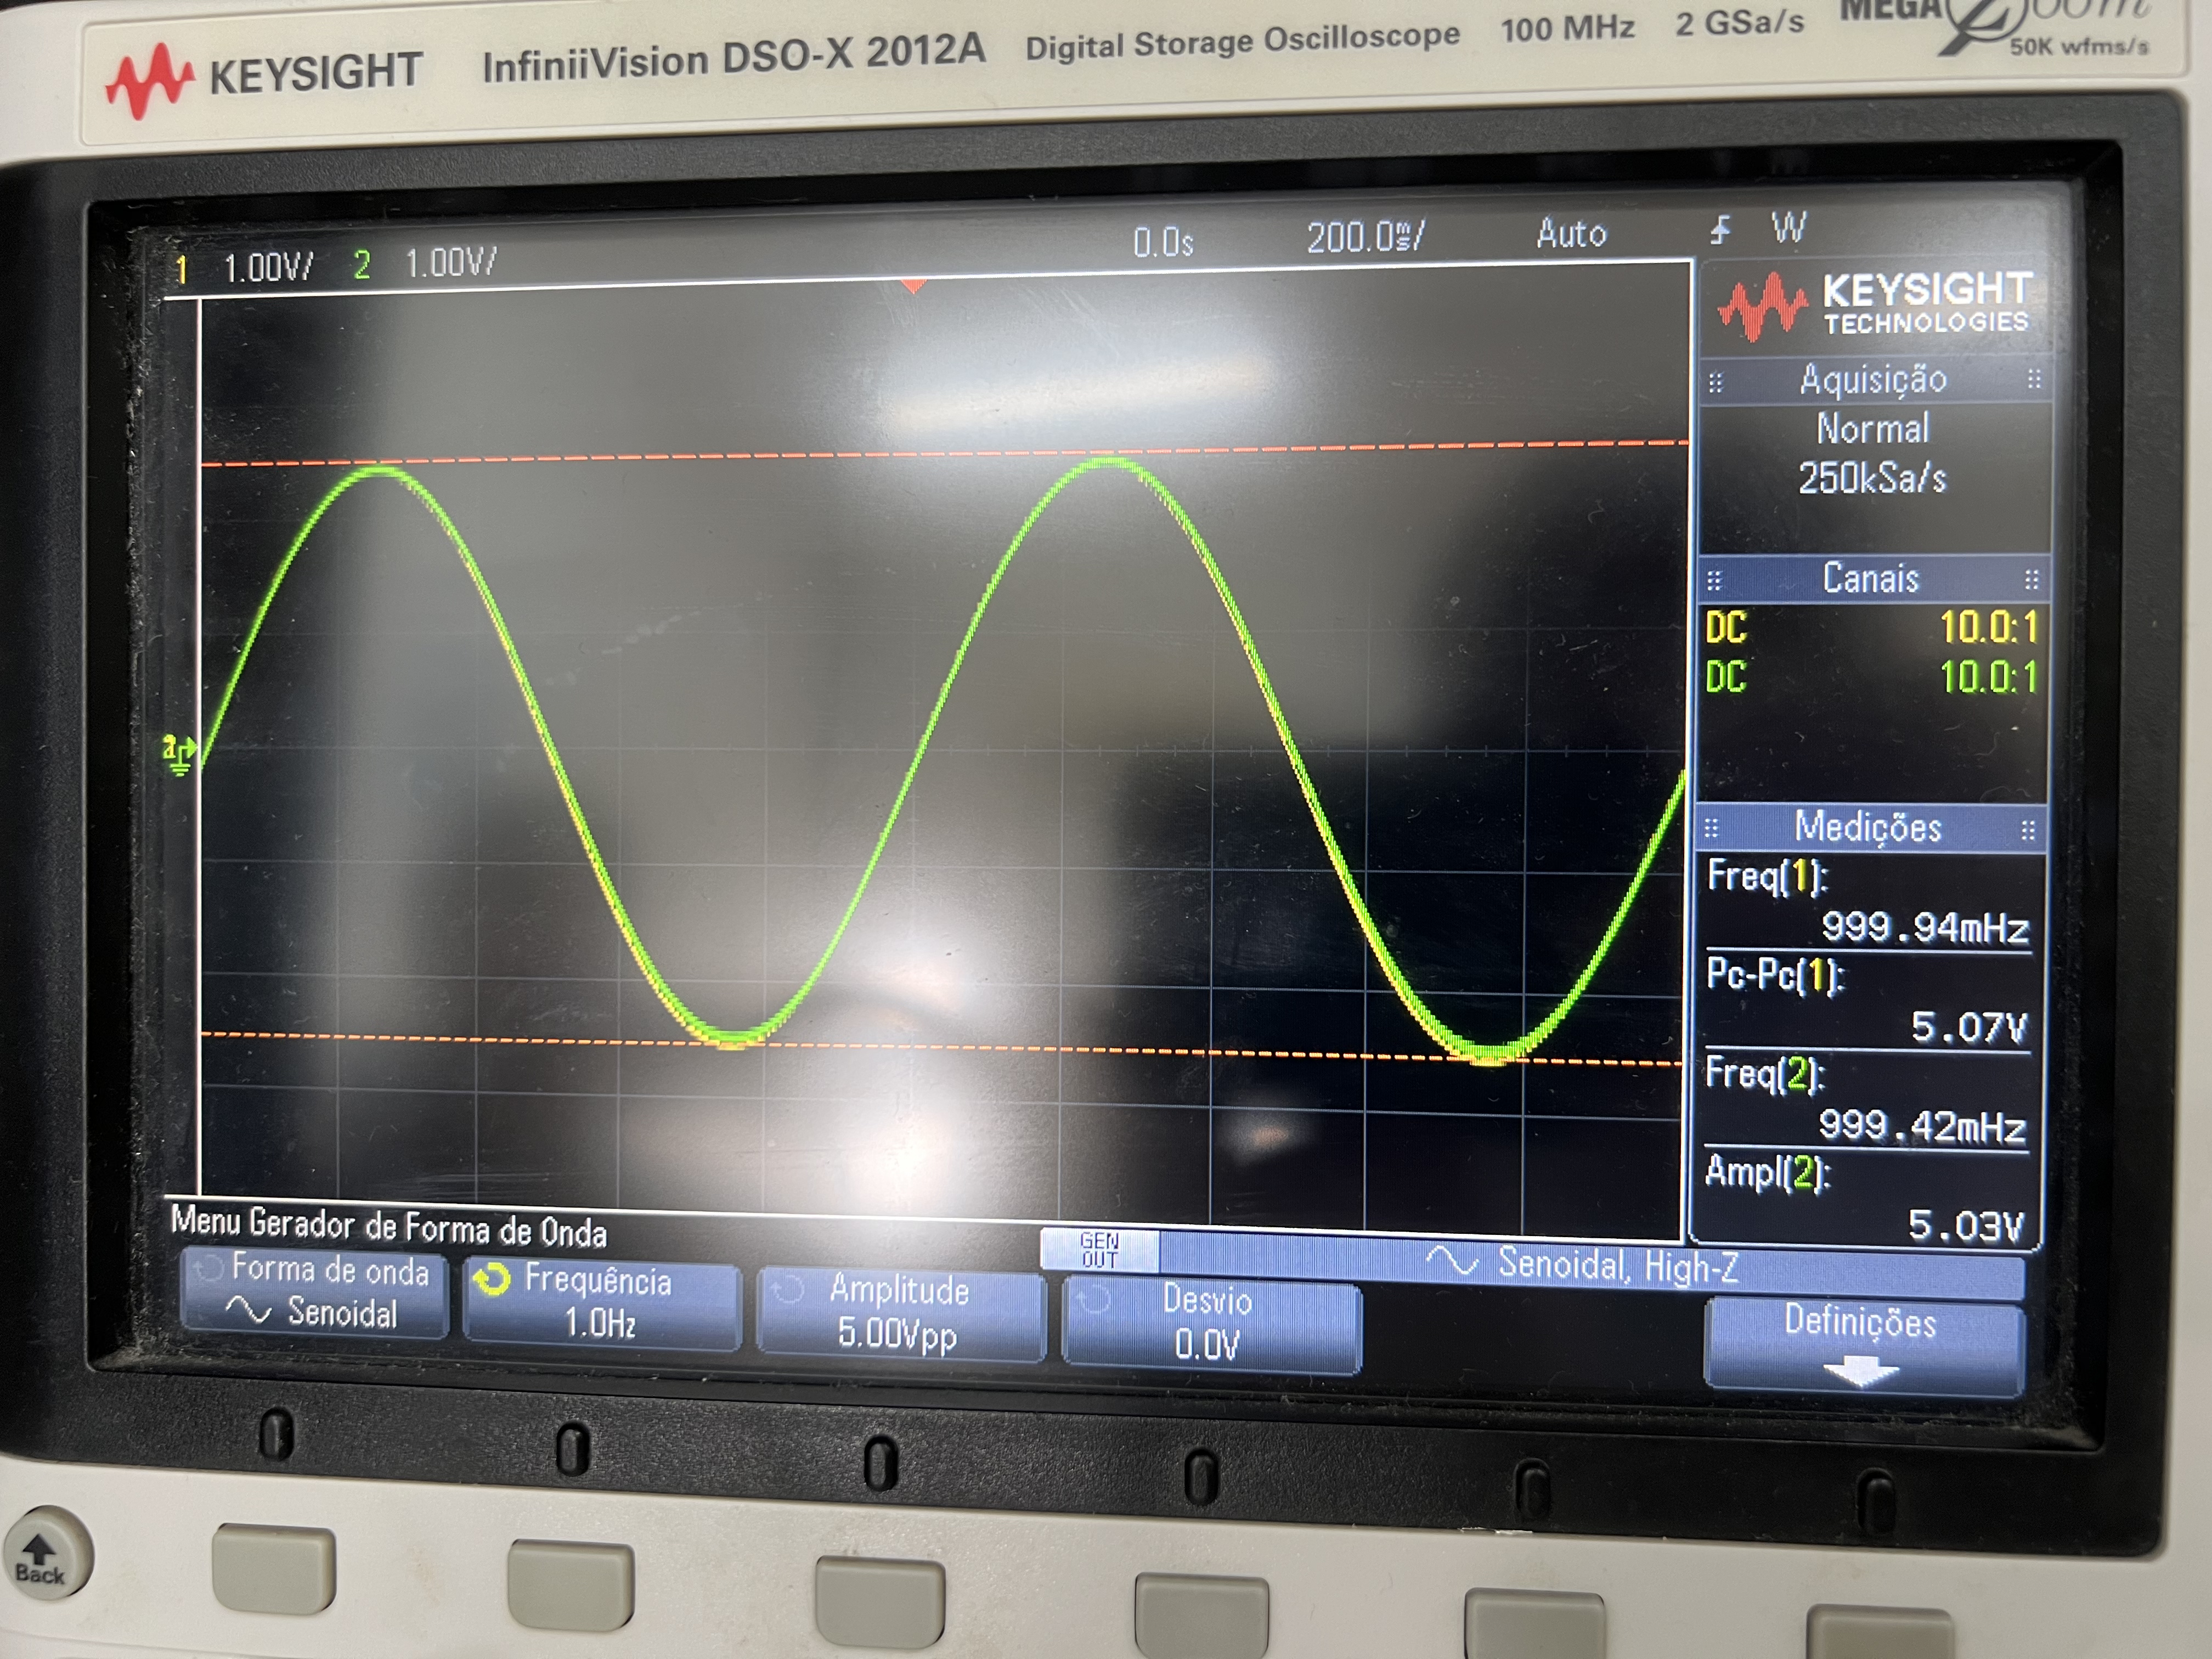
\includegraphics[width=1\columnwidth]{images/osciloscopio/circuito1_ganho.png}
    \caption{Ganho do Circuito 1 a baixas frequências.}
\end{figure}


\subparagraph{Podemos observar que o ganho do circuito 1 foi $1$.}


\pagebreak


\subsection{Frequência de corte}


\begin{figure}[h]
    \centering
    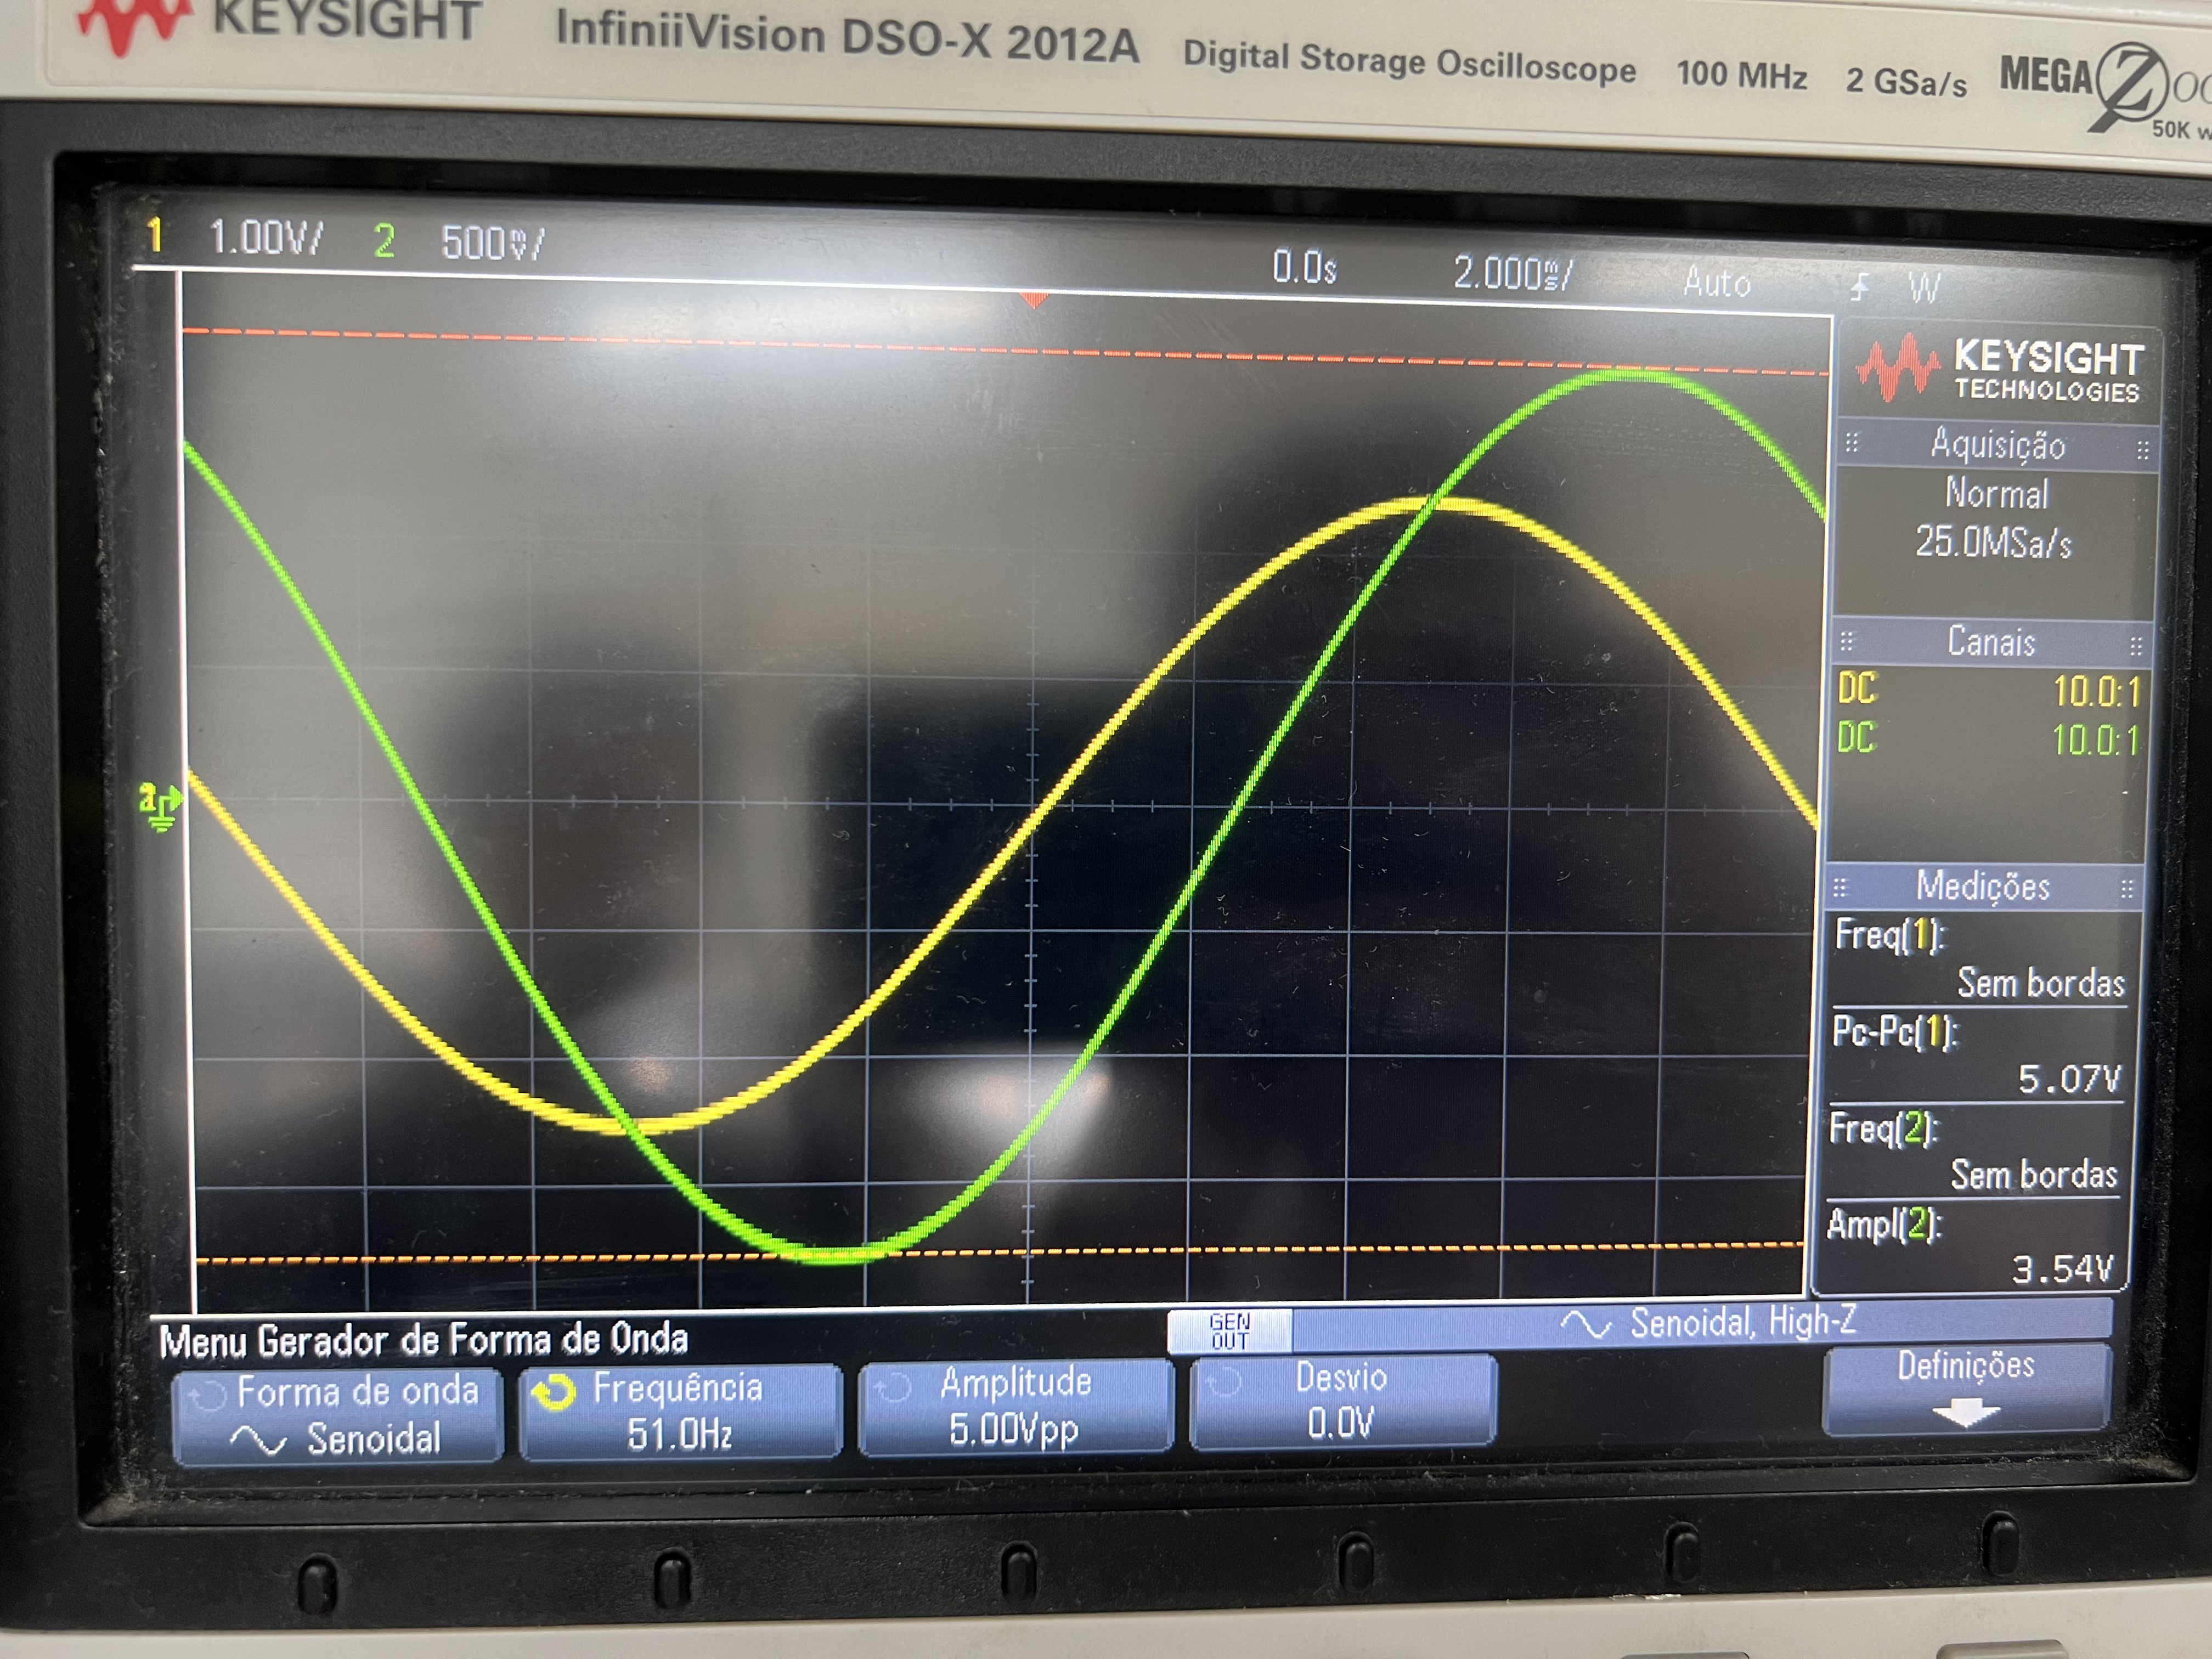
\includegraphics[width=1\columnwidth]{images/osciloscopio/circuito1_freqcorte.png}
    \caption{Frequência de corte do Circuito 1.}
\end{figure}


\subparagraph{Sua frequência de corte foi $51Hz$, já que esta será obtida quando tivermos aproximadamente $\frac{V_i * ganho}{\sqrt[]{2}} = 3.53V$ que é próximo do valor esperado da análise numérica que foi de $50Hz$.}


\subsection{Resultados das medidas}
\begin{center}
    \begin{tabular}{ |c|c|c|c| }
        \hline
        Múltiplos & Freq (Hz) & Entrada (V) & Saída (V) \\
        0.02      & $1$       & $5.07$      & $5.03$    \\
        0.2       & $10.2$    & $5.07$      & $4.78$    \\
        0.5       & $25.5$    & $5.07$      & $4.44$    \\
        0.75      & $38.2$    & $5.07$      & $4.06$    \\
        1.25      & $63.8$    & $5.07$      & $3.24$    \\
        1.6       & $81.6$    & $5.07$      & $2.77$    \\
        2.5       & $127.5$   & $5.07$      & $1.94$    \\
        3.5       & $178.5$   & $5.07$      & $1.46$    \\
        5         & $255$     & $5.07$      & $1.04$    \\
        10        & $510$     & $5.07$      & $0.521$   \\
        20        & $1020$    & $5.07$      & $0.27$    \\
        \hline
    \end{tabular}
\end{center}


\newpage


\subsection{O Circuito 2}


\paragraph{Vamos inicialmente fazer as medições dos componentes a serem usados.}


\subsection{Tabela de componentes}


\begin{equation*}
    \begin{aligned}
        C_1 & = 95.78nF         \\
        R_1 & = 46.6k \varOmega \\
        R_L & = 21.9k
    \end{aligned}
\end{equation*}


\subsection{Ganho em frequências baixas}


\begin{figure}[h]
    \centering
    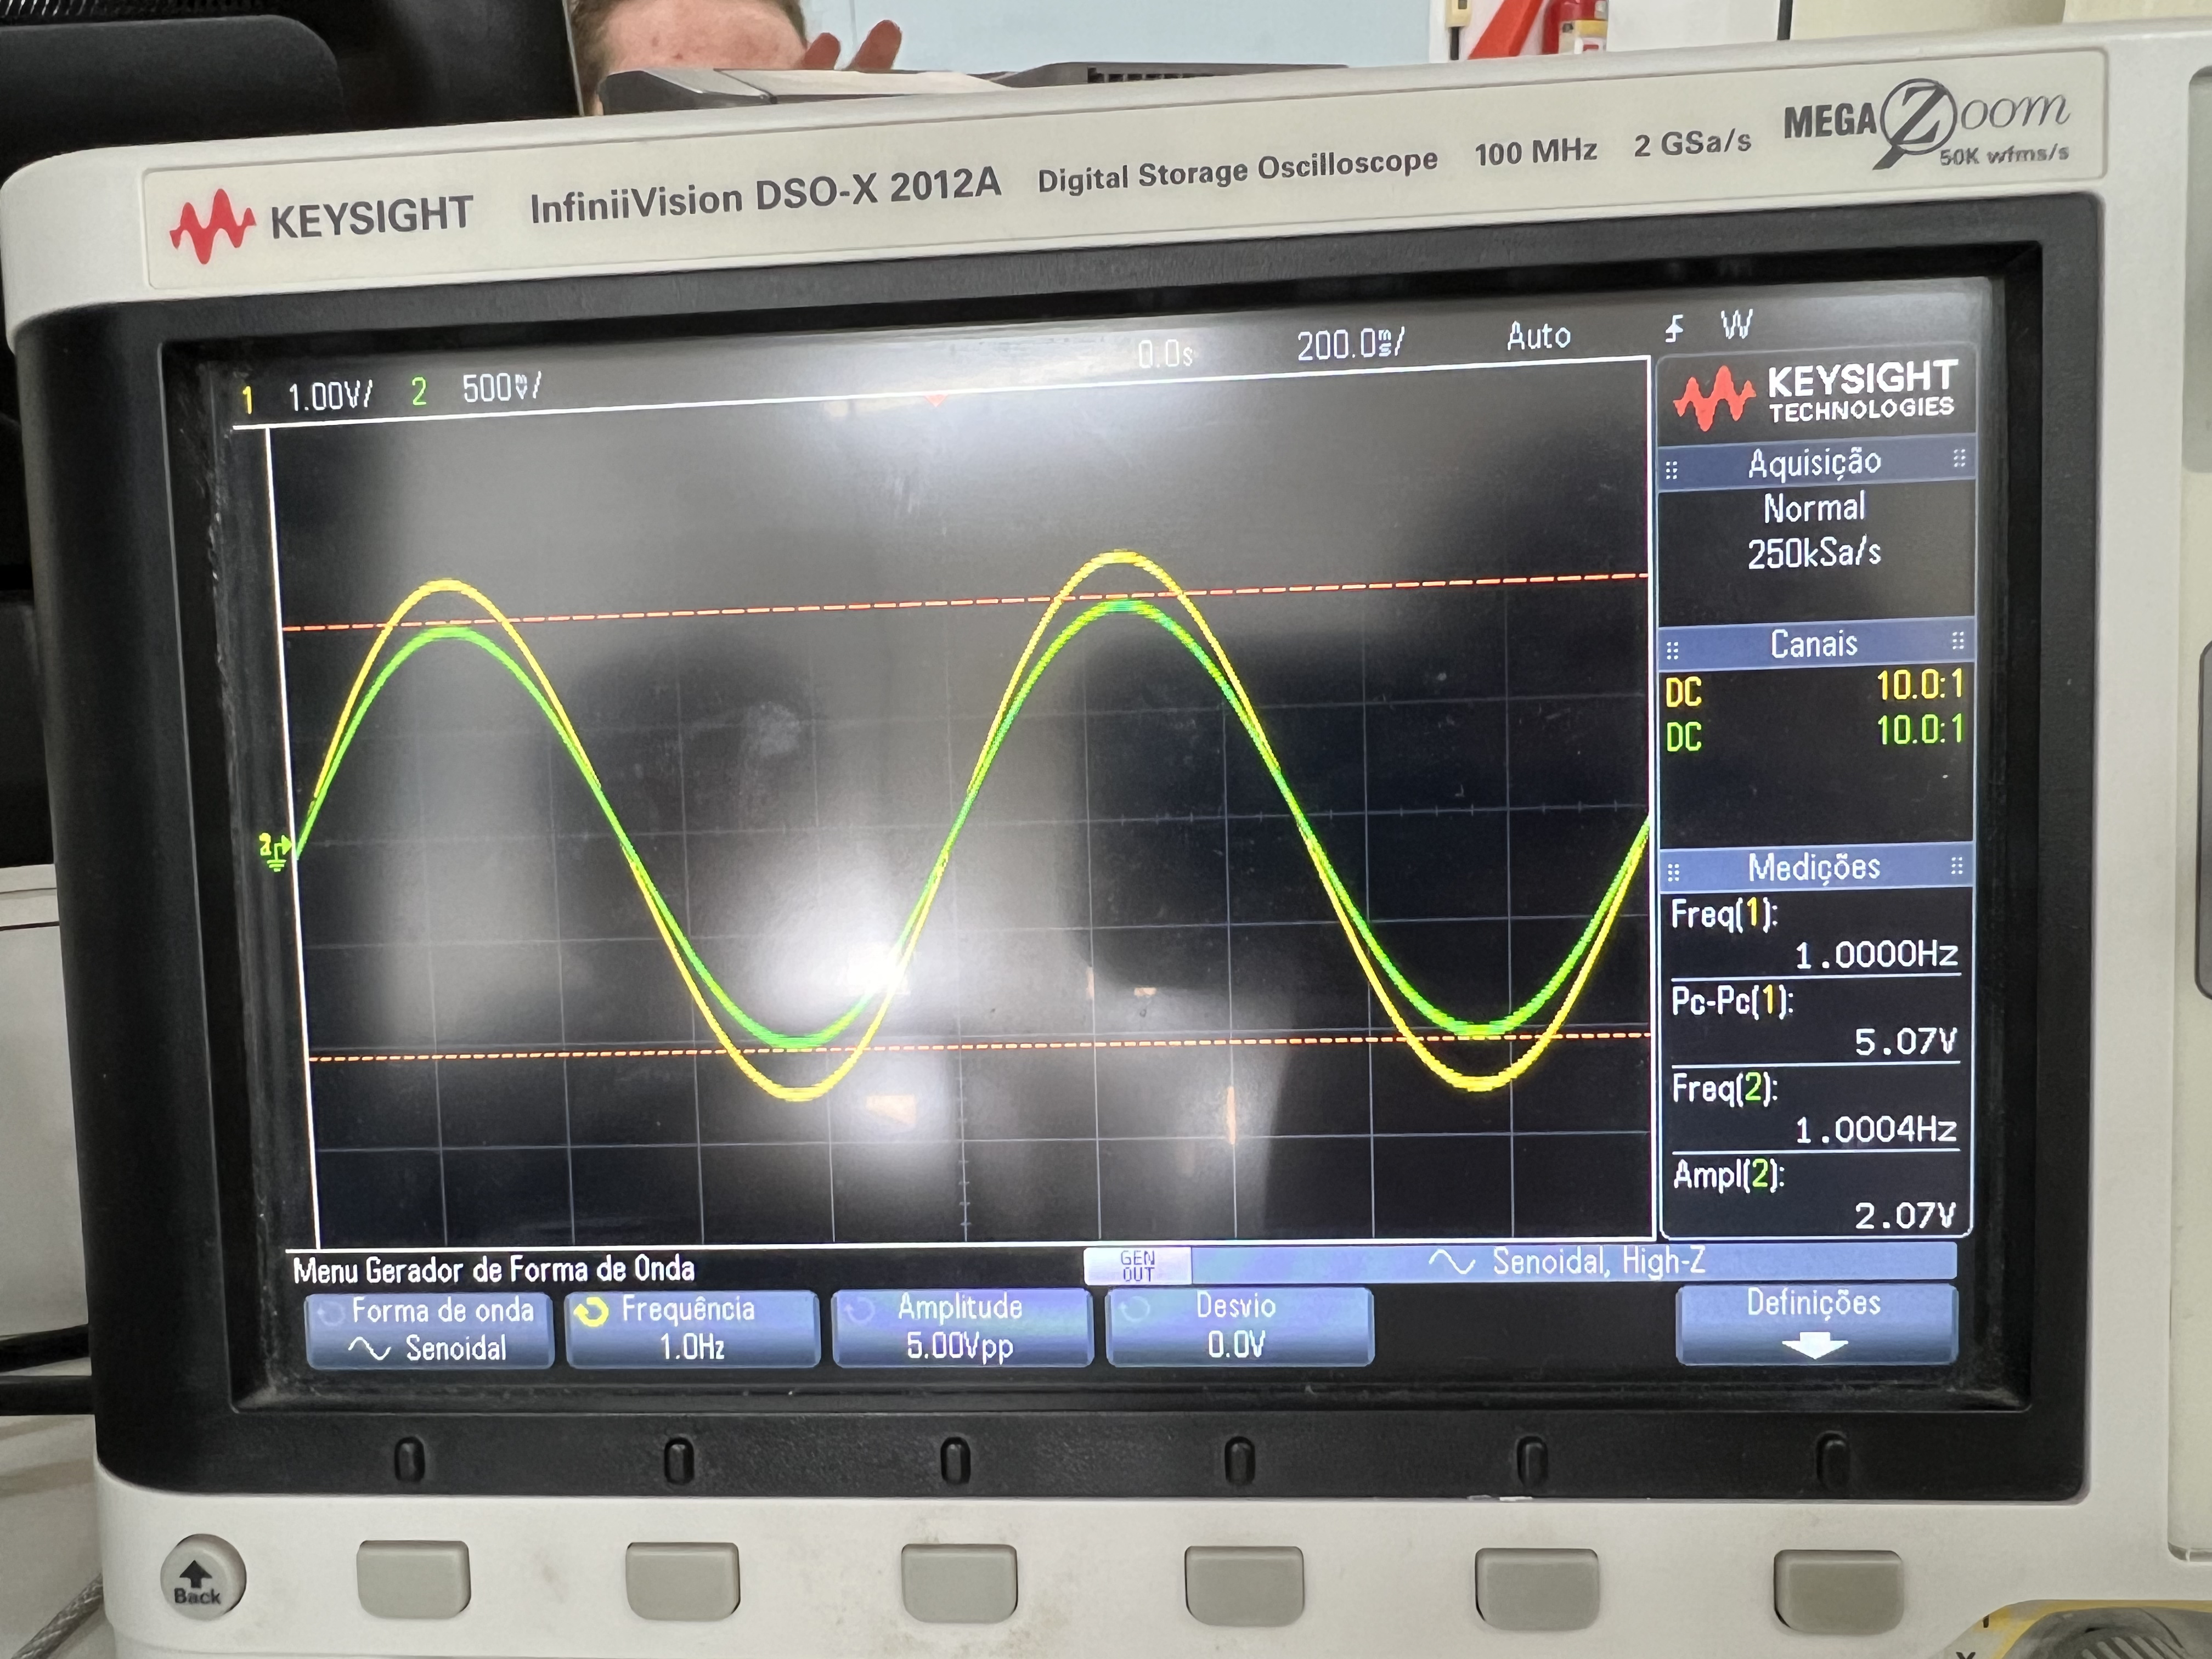
\includegraphics[width=1\columnwidth]{images/osciloscopio/circuito2_ganho.png}
    \caption{Ganho do Circuito 2 a baixas frequências.}
\end{figure}


\subparagraph{Podemos observar que o ganho do circuito 2 foi $0.4$.}




\subsection{Frequência de corte}


\begin{figure}[h]
    \centering
    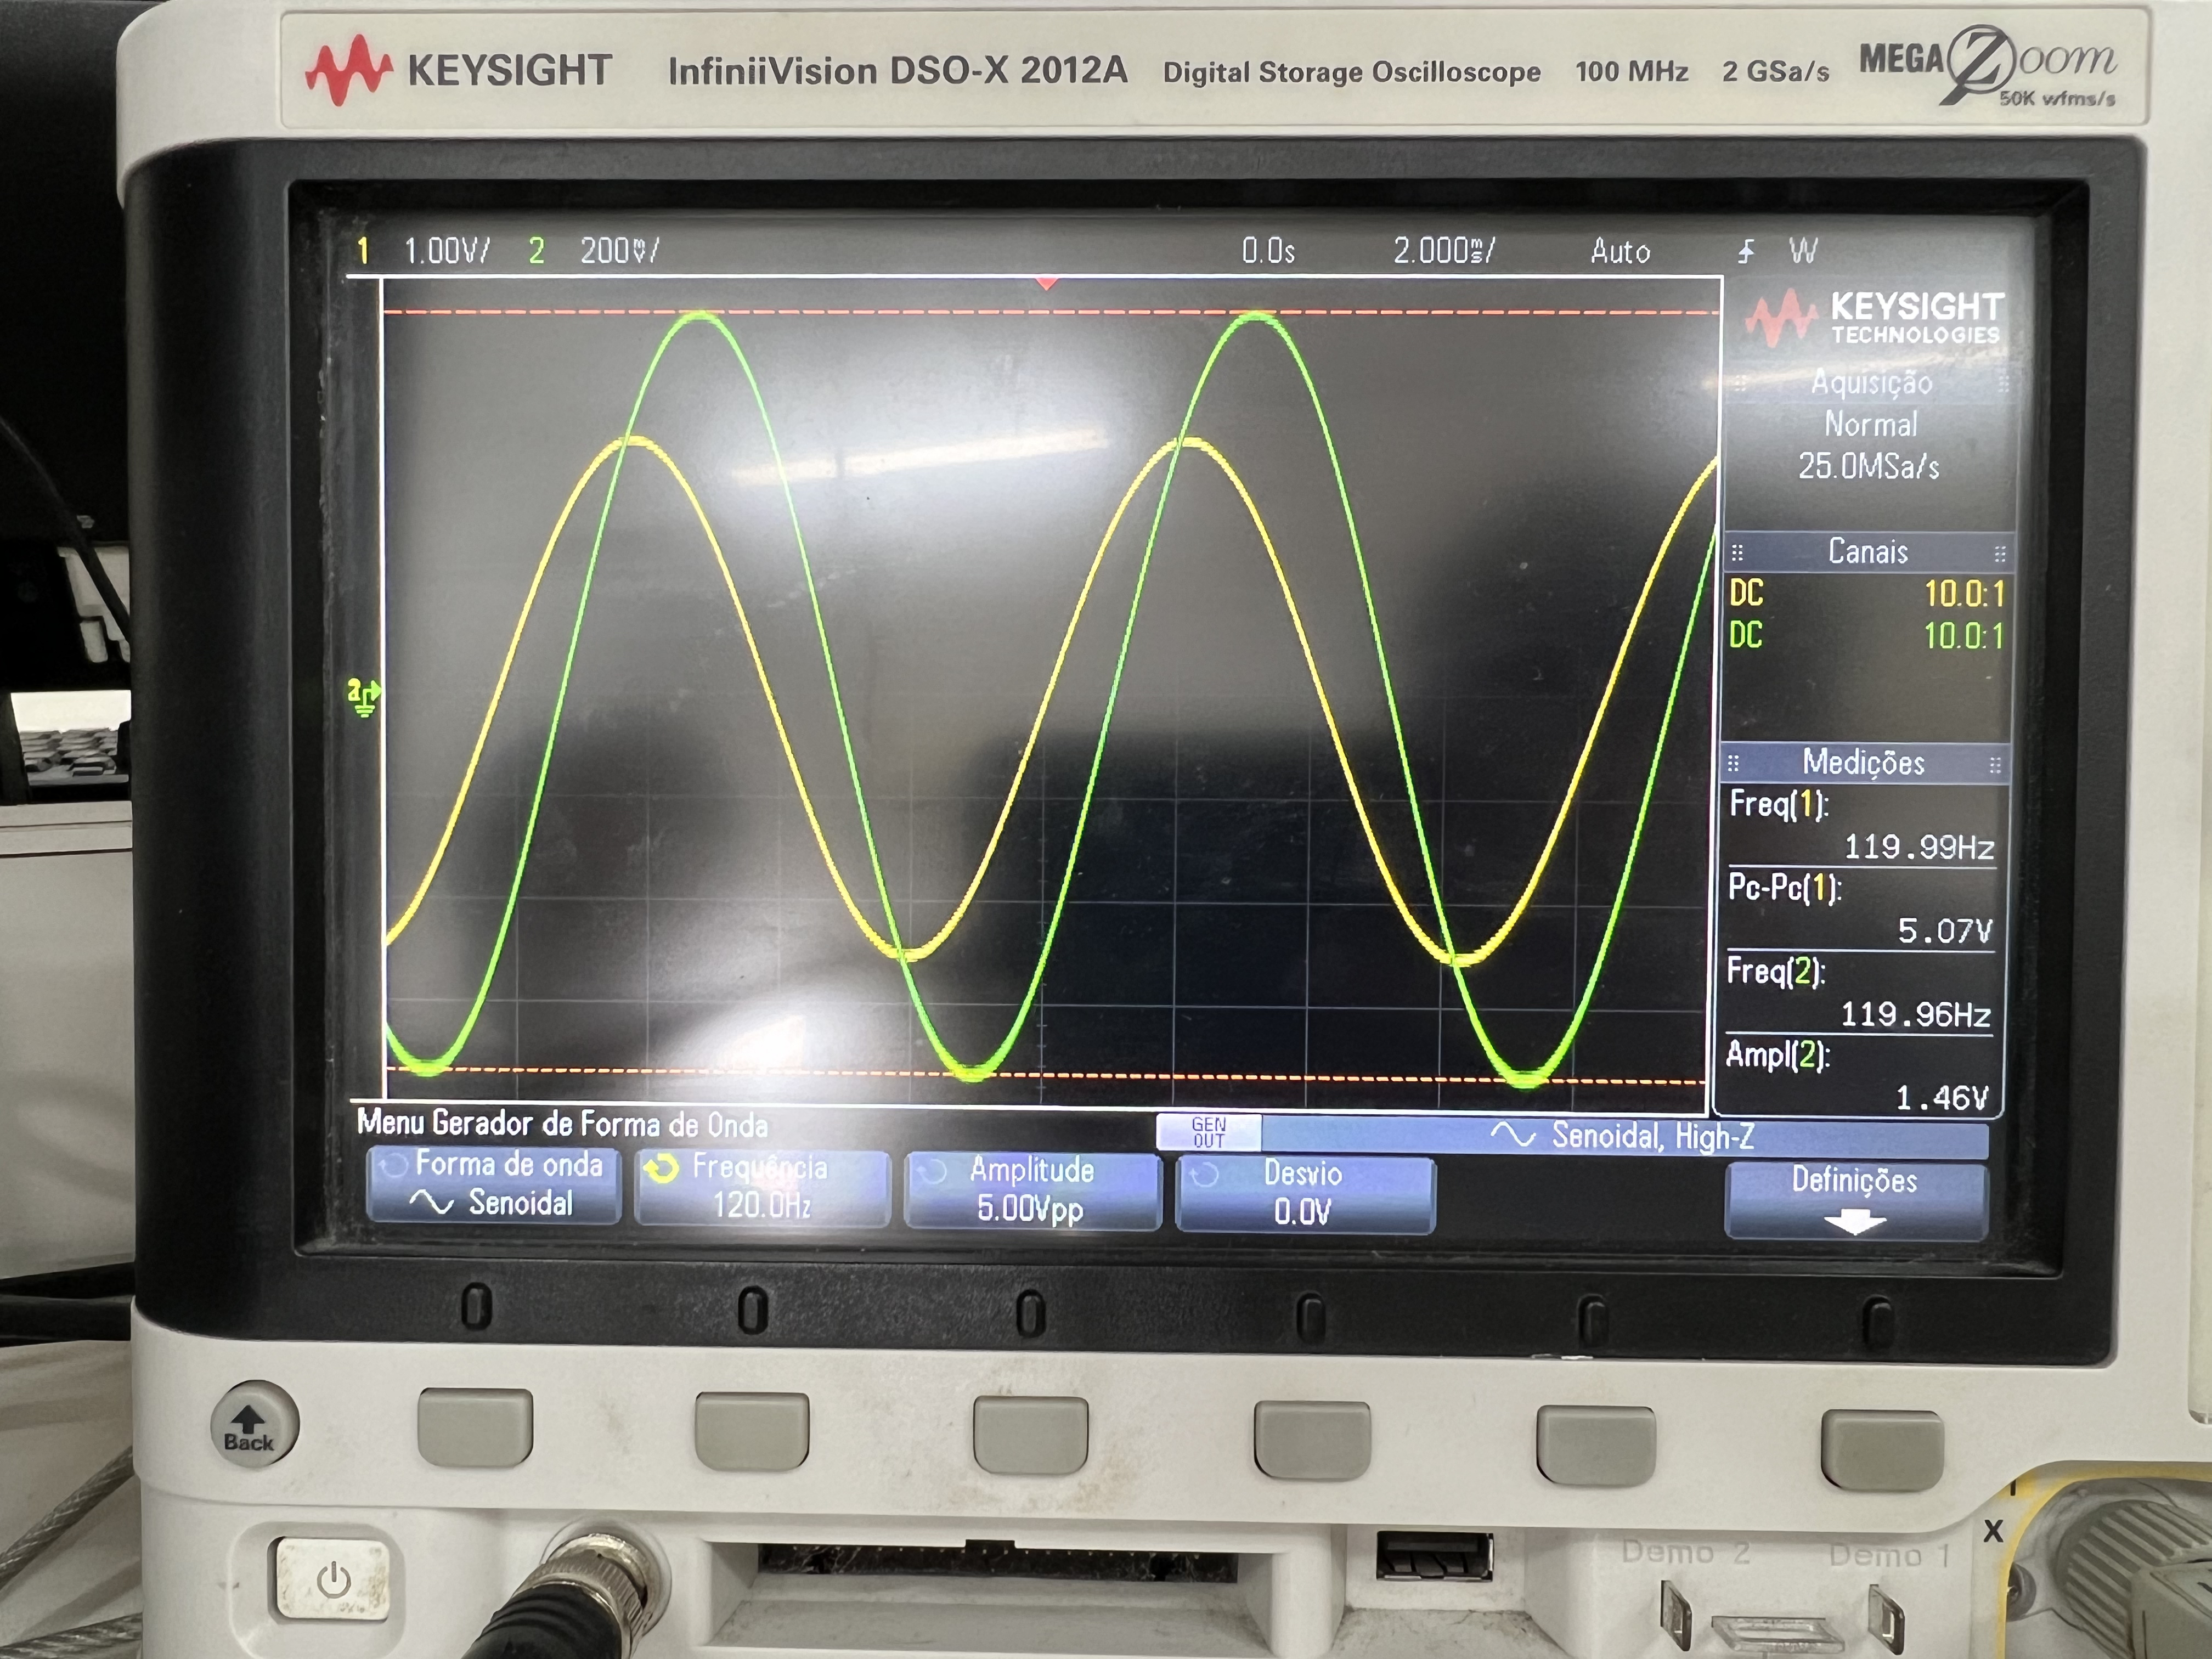
\includegraphics[width=1\columnwidth]{images/osciloscopio/circuito2_freqcorte.png}
    \caption{Frequência de corte do Circuito 2.}
\end{figure}


\subparagraph{Sua frequência de corte foi $120Hz$, já que esta será obtida quando tivermos aproximadamente $\frac{V_i * ganho}{\sqrt[]{2}} = 1.42V$ que é próximo do valor esperado da análise numérica que foi de $120Hz$.}


\subsection{Resultados das medidas}
\begin{center}
    \begin{tabular}{ |c|c|c|c| }
        \hline
        Múltiplos & Freq (Hz) & Entrada (V) & Saída (V) \\
        0.02      & $1$       & $5.07$      & $2.07$    \\
        0.2       & $24$      & $5.07$      & $2$       \\
        0.5       & $60$      & $5.07$      & $1.89$    \\
        0.75      & $90$      & $5.07$      & $1.71$    \\
        1.25      & $150$     & $5.07$      & $1.29$    \\
        1.6       & $192$     & $5.07$      & $1.1$     \\
        2.5       & $300$     & $5.07$      & $0.835$   \\
        3.5       & $420$     & $5.07$      & $0.601$   \\
        5         & $600$     & $5.07$      & $0.44$    \\
        10        & $1200$    & $5.07$      & $0.26$    \\
        20        & $2400$    & $5.07$      & $0.15$    \\
        \hline
    \end{tabular}
\end{center}


\newpage


\subsection{O Circuito 3}


\paragraph{Vamos inicialmente fazer as medições dos componentes a serem usados.}


\subsection{Tabela de componentes}


\begin{equation*}
    \begin{aligned}
        C_1 & = 95.78nF         \\
        R_1 & = 46.6k \varOmega \\
        R_L & = 21.9k
    \end{aligned}
\end{equation*}


\subsection{Ganho em frequências baixas}


\begin{figure}[h]
    \centering
    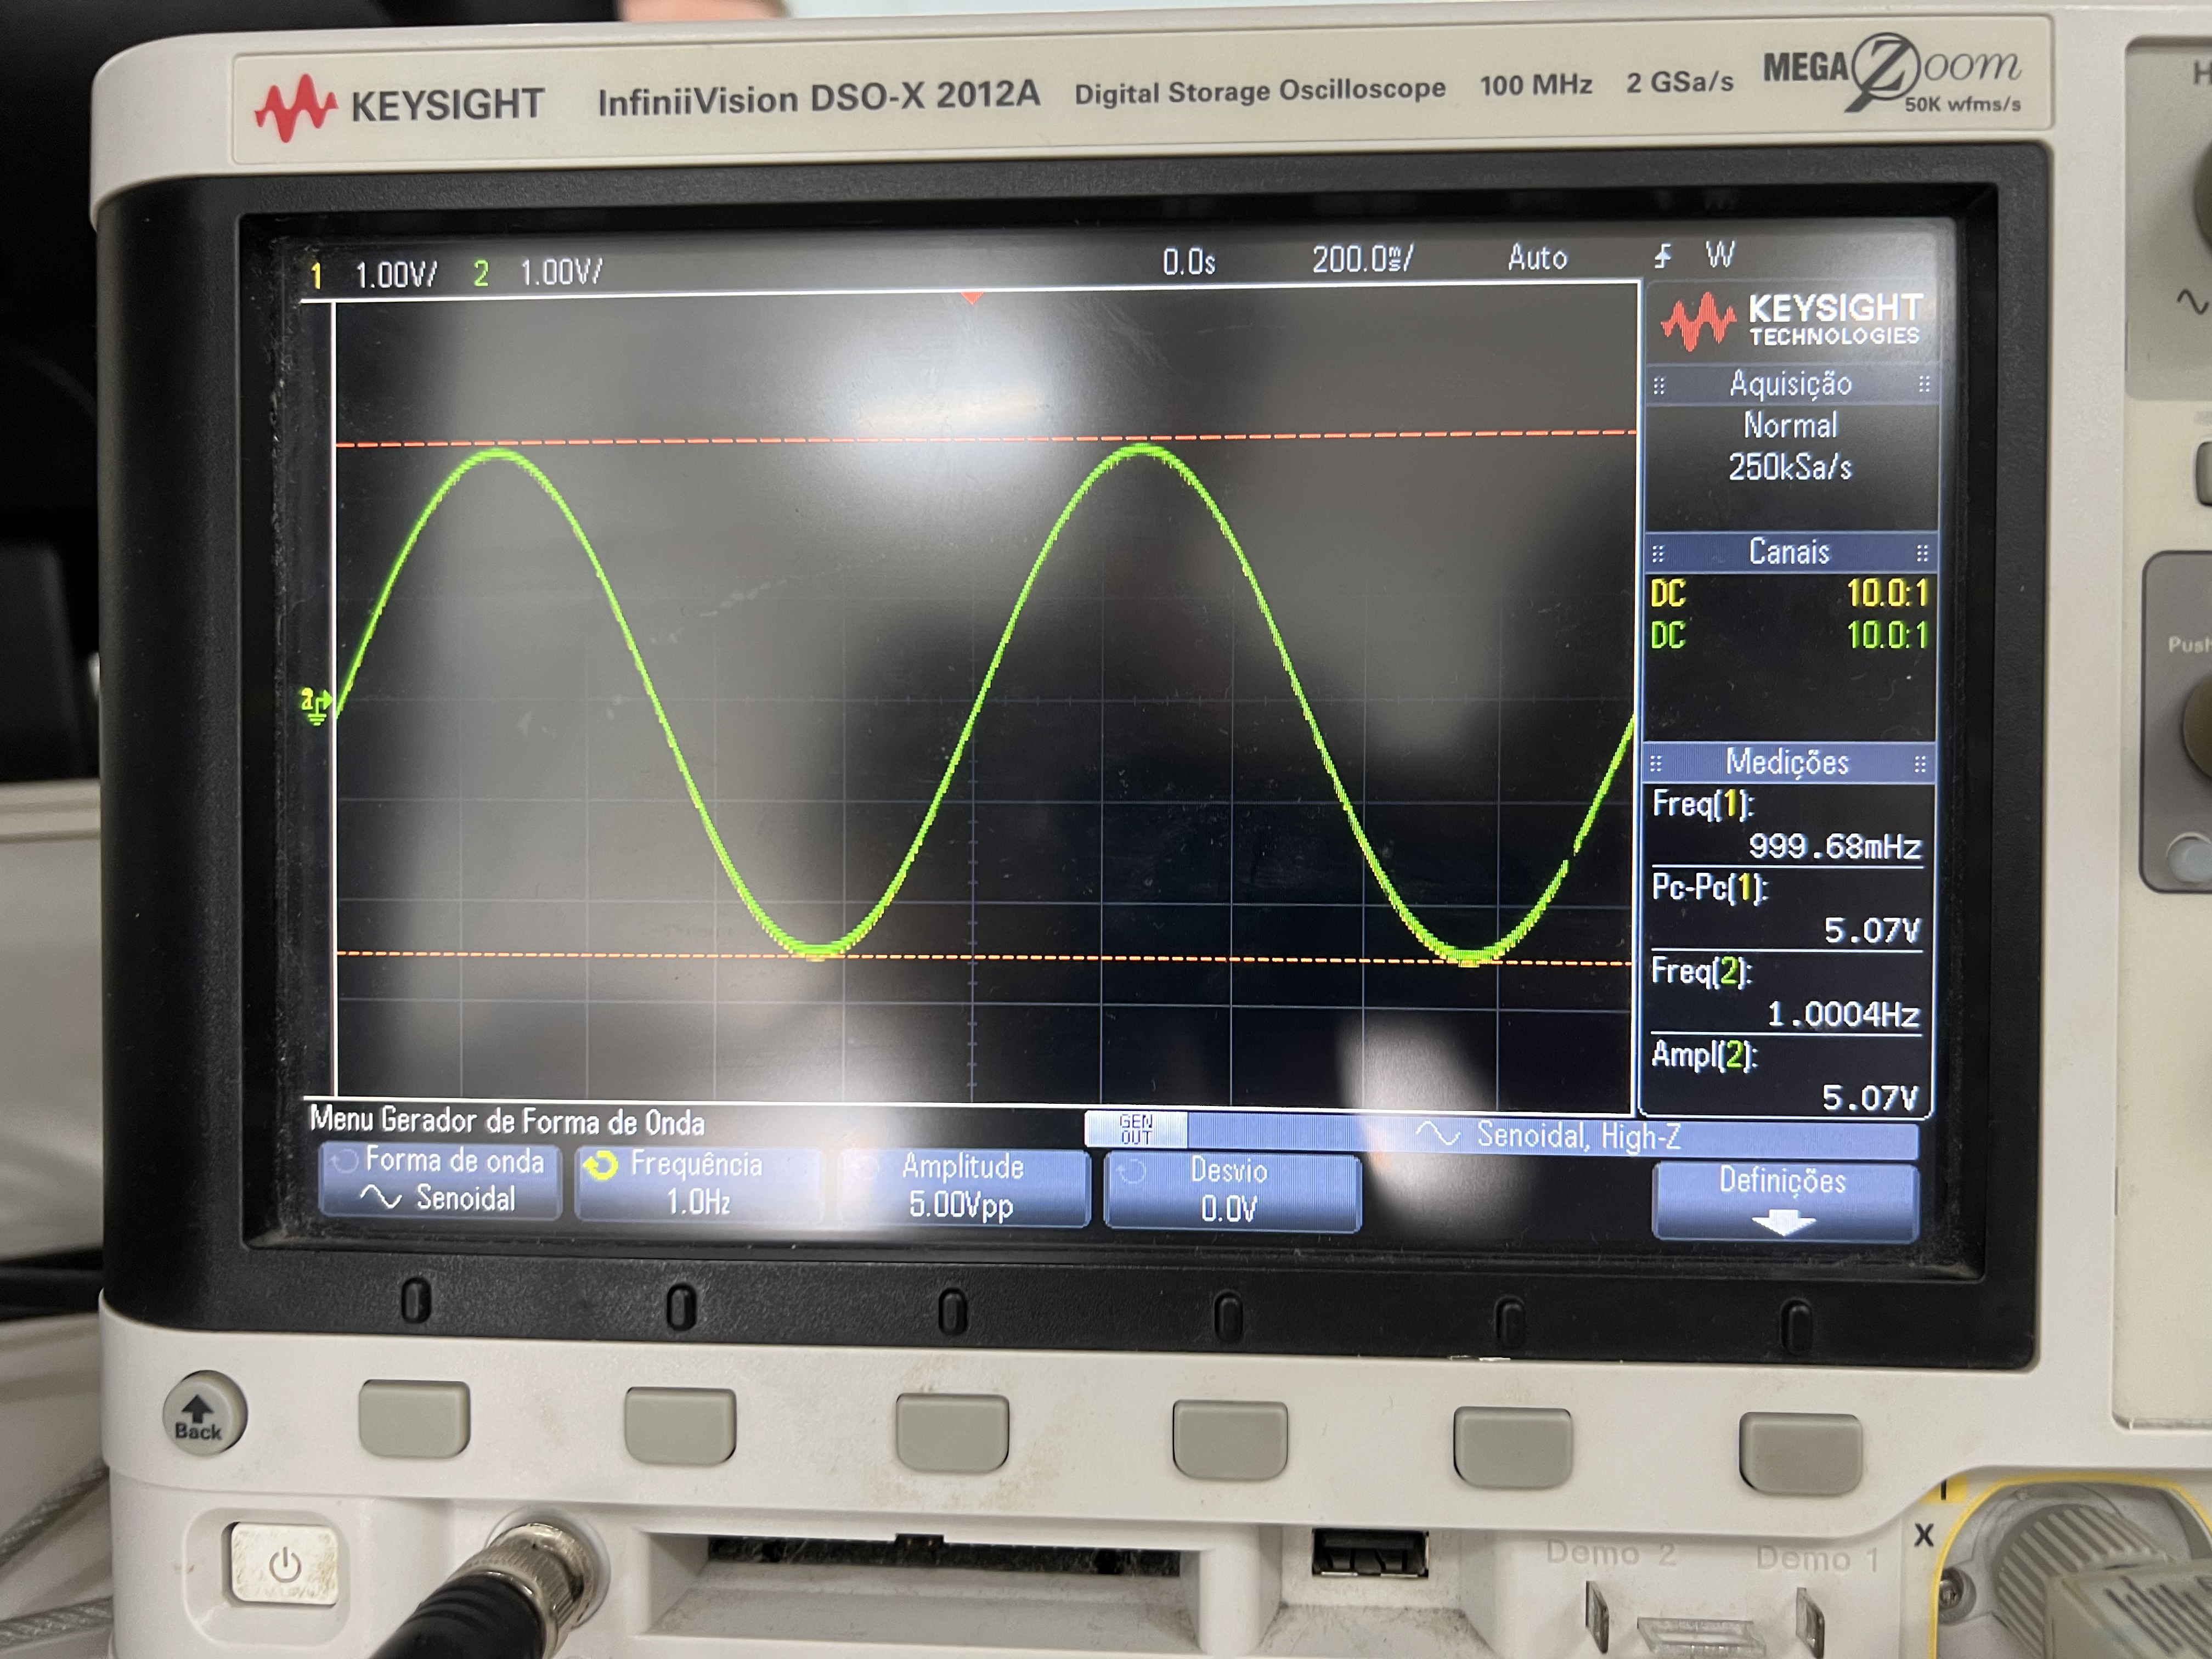
\includegraphics[width=1\columnwidth]{images/osciloscopio/circuito3_ganho.png}
    \caption{Ganho do Circuito 3 a baixas frequências.}
\end{figure}


\subparagraph{Podemos observar que o ganho do circuito 3 foi $1$.}




\subsection{Frequência de corte}


\begin{figure}[h]
    \centering
    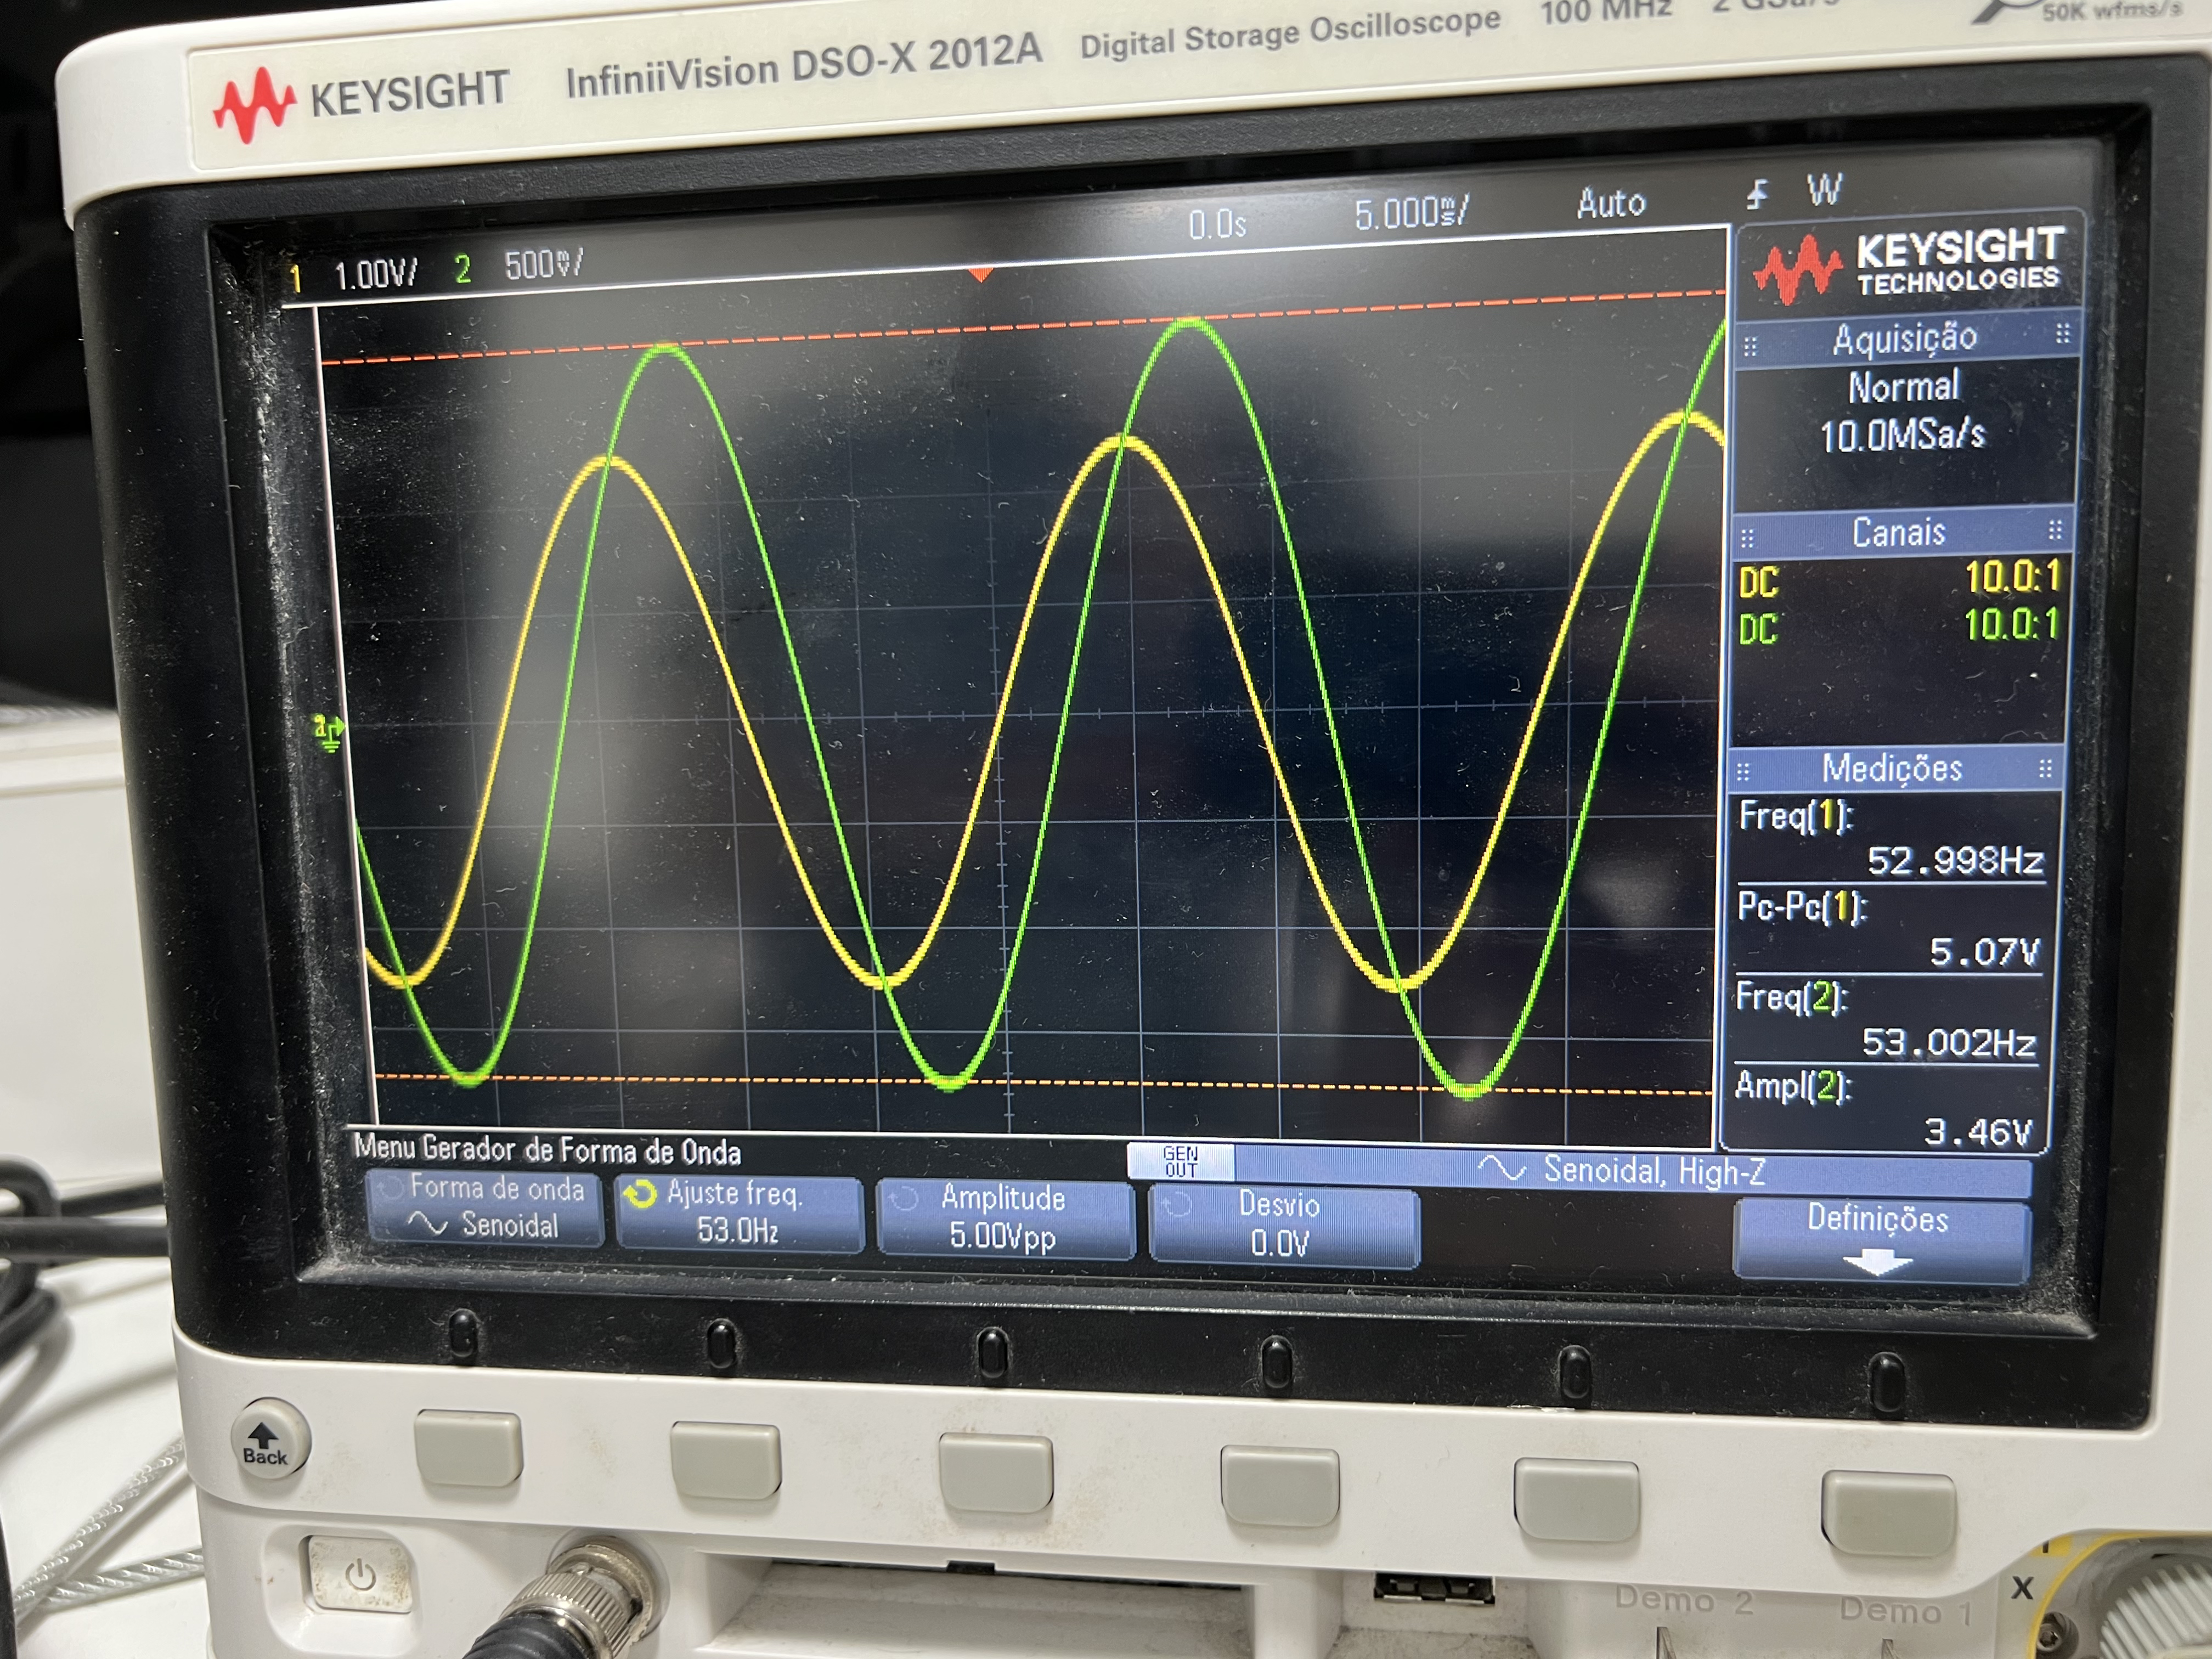
\includegraphics[width=1\columnwidth]{images/osciloscopio/circuito3_freqcorte.png}
    \caption{Frequência de corte do Circuito 3.}
\end{figure}


\subparagraph{Sua frequência de corte foi $53Hz$, já que esta será obtida quando tivermos aproximadamente $\frac{V_i * ganho}{\sqrt[]{2}} = 3.56V$ que é próximo do valor esperado da análise numérica que foi de $50Hz$.}


\subparagraph*{Interessantemente, esta frequência de corte ficou acima da frequência de corte do circuito 1, que foi de $51Hz$. Creio que por erros de medição.}


\subsection{Resultados das medidas}
\begin{center}
    \begin{tabular}{ |c|c|c|c| }
        \hline
        Múltiplos & Freq (Hz) & Entrada (V) & Saída (V) \\
        0.02      & $1$       & $5.07$      & $5.07$    \\
        0.2       & $10.6$    & $5.07$      & $4.94$    \\
        0.5       & $26.5$    & $5.07$      & $4.5$     \\
        0.75      & $39.75$   & $5.07$      & $4.04$    \\
        1.25      & $66.25$   & $5.07$      & $3.06$    \\
        1.6       & $84.8$    & $5.07$      & $2.57$    \\
        2.5       & $132.5$   & $5.07$      & $1.87$    \\
        3.5       & $185.5$   & $5.07$      & $1.33$    \\
        5         & $265$     & $5.07$      & $0.965$   \\
        10        & $530$     & $5.07$      & $0.513$   \\
        20        & $1060$    & $5.07$      & $0.258$   \\
        \hline
    \end{tabular}
\end{center}


\newpage


\section{Pós-laboratorial}


\subparagraph*{Reutilizei o código do Maxima para calcular a frequência de corte e ganho dos circuitos, e obtive os seguintes resultados:}




\subsection{Circuito 1}


\begin{figure}[h]
    \centering
    \includegraphics[width=1\columnwidth]{images/circuito1_freqreal.png}
    \caption{Cálculo de ganho e frequência de corte para Circuito 1.}
\end{figure}


\subparagraph*{Daí vemos que temos ganho de $1$ e frequência de corte de $51.4Hz$. Que está bem próxima da frequência de $51Hz$ que encontramos experimentalmente.}


\begin{figure}[h]
    \centering
    \includegraphics[width=1\columnwidth]{images/circuito1wx.png}
    \caption{Gráfico log-log do ganho em função da frequência do Circuito 1.}
\end{figure}


\pagebreak
\newpage


\subsection{Circuito 2}


\begin{figure}[h]
    \centering
    \includegraphics[width=1\columnwidth]{images/circuito2_freqreal.png}
    \caption{Cálculo de ganho e frequência de corte para Circuito 2.}
\end{figure}


\subparagraph*{Daí vemos que temos ganho de $0.404$ e frequência de corte de $127.2Hz$. Que está bem próxima da frequência de $120Hz$ que encontramos experimentalmente.}


\begin{figure}[h]
    \centering
    \includegraphics[width=1\columnwidth]{images/circuito2wx.png}
    \caption{Gráfico log-log do ganho em função da frequência do Circuito 2.}
\end{figure}


\pagebreak
\newpage


\subsection{Circuito 3}


\subparagraph*{Como já havíamos discutido anteriormente, a análise teórica para o circuito 3 é igual a análise teórica vista acima para o circuito 1. Então este terá os mesmos valores de ganho de $1$ e frequência de corte de $51.4Hz$.}


\subparagraph*{Vale a pena reparar que apesar da análise teórica para ambos circuitos ser a mesma, os resultados obtidos experimentalmente foram ligeiramente diferentes, provavelmente devido a erros de medição.}


\begin{figure}[h]
    \centering
    \includegraphics[width=1\columnwidth]{images/circuito3wx.png}
    \caption{Gráfico log-log do ganho em função da frequência do Circuito .}
\end{figure}


\newpage


\section{Conclusões}


\subparagraph*{Conseguimos com sucesso fazer a análise numérica pelo WxMaxima, e comparamos os resultados com os obtidos experimentalmente.}




\subparagraph*{Nos resultados práticos, a magnitude da função transferência e as frequências de corte foram coerentes com os resultados esperados.}


\subparagraph*{Os gráficos que geramos a partir dos resultados experimentais foram coerentes com os gráficos gerados numericamente}


\subparagraph*{Em suma creio que tivemos sucesso em nos familiarizar com as ferramentas de análise de circuitos elétricos numéricos.}


\end{document}